\section{Homeostasis of the Community with Markov Chain Model}\label{sec:markov}

% TODO: Cite references

\subsection{Feasibility of utilizing Markov chain model in fungus community}

Since it is presumably impractical for finding the symbolic solution of the LV model, Markov chain model is introduced for predicting the stable state, that is, the relatively static composition of the fungus populations density in the community.

\begin{definition}
    Once the community component is stabilized, if possible, the population density of each fungi specie interchange in a rate proportional to its own population density, the coefficient is a constant.
\end{definition}

\paragraph{Justification} Though the Markov chain model is based on discrete time and state space, since the stable state is all we concerned in this attempt, we can still utilize such notion.

\begin{figure}\caption{A Markov chain diagram containing 3 fungi species}\label{fig:markov3}
    \begin{center}
        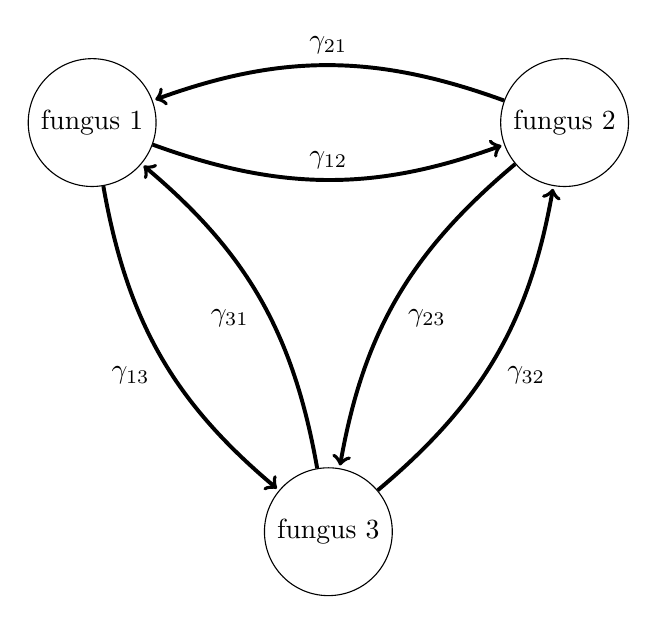
\begin{tikzpicture}
            \node[draw, circle] at (0, 0)     (1)     {fungus 1};
            \node[draw, circle] at (6, 0)     (2)     {fungus 2};
            \node[draw, circle] at (3, -5.196) (3) {fungus 3};
    
            \draw[every loop, auto=right, line width=0.5mm]
                (1) edge[bend right=20]            node {$\gamma_{13}$} (3)
                (1) edge[bend right=20, auto=left] node {$\gamma_{12}$} (2)
                (2) edge[bend right=20]            node {$\gamma_{21}$} (1)
                (2) edge[bend right=20, auto=left] node {$\gamma_{23}$} (3)
                (3) edge[bend right=20]            node {$\gamma_{32}$} (2)
                (3) edge[bend right=20, auto=left] node {$\gamma_{31}$} (1);
        \end{tikzpicture}
    \end{center}
\end{figure}


\subsection{Constructing Markov chain for fungus community}

Consider a given time interval $T$, and the population density of each fungus species at time $t$ is denoted as $\boldsymbol{x}(t) = [x_1(t), x_2(t), \cdots, x_n(t)]^T$. In the evolution process of the community, at each time interval, a specific percentage of fungi $i$ is remained, and others can be considered as transformed into population density of other species of fungus.

For a simple dual-species system, such transition relation can be expressed as

\begin{equation}
    \left\{\begin{aligned} &
        x_1(t+T) = \gamma_{11}x_1(t) + \gamma_{21}x_2(t) \\ &
        x_2(t+T) = \gamma_{22}x_2(t) + \gamma_{12}x_1(t)
    \end{aligned}\right..
\end{equation}

More generally, in an $n$-species community, the system is characterized by

\begin{equation}
    \left\{\begin{aligned} &
        x_1(t+T) = \gamma_{11}x_1(t) + \cdots + \gamma_{n1}x_n(t) \\ & \cdots \\ &
        x_i(t+T) = \sum_{j=1}^n \gamma_{ij}x_j \\ & \cdots \\ &
        x_n(t+T) = \gamma_{n1}x_1(t) + \cdots + \gamma_{nn}x_n(t).
    \end{aligned}\right.
\end{equation}

Which can be further simplified with matrix notation.

\begin{equation}\label{eq:trans}
    \boldsymbol{x}(t+T) = \boldsymbol{x}(t)\boldsymbol{Y}.
\end{equation}

In which, the matrix $\boldsymbol{Y}_{n\times n}$ is defined to be the transition matrix of the system, with element $\gamma_{ij}$ denoting the transition rate from fungus specie $i$ to $j$.

\begin{equation}
    \boldsymbol{Y} =
    \begin{bmatrix}
        \gamma_{11} & \gamma_{12} & \cdots & \gamma_{1n} \\
        \gamma_{21} & \ddots & & \vdots \\
        \vdots & & \ddots & \vdots \\
        \gamma_{n1} & \cdots & \cdots & \gamma_{nn}
    \end{bmatrix}
\end{equation}

Note that the transition rate in the biological configuration considerably differs from that in stochastic process. In a typical Markov chain model, each element in the transition matrix represents a certain probability of transition or decision towards another state. To implement this model in a continuous mathematical configuration, adjustments must be and evidently can be made to the definition of the population density $x_i$ itself, ensuring that a unit of population density of different species of fungus takes up the same amount of resources in the system. With such adjustment, it is guaranteed that, for each element and row of the transition matrix, we have

\begin{equation}\label{eq:markov-norm}
    \left\{\begin{aligned} &
        \boldsymbol{Y}_{ij} \in [0,\ 1],\ i,\ j\in\{1,\ 2,\ \cdots,\ n\} \\ &
        \sum_{j=1}^n \boldsymbol{Y}_{ij} = 1,\ i\in\{1,\ 2,\ \cdots,\ n\}.
    \end{aligned}\right.
\end{equation}

In addition, though during the growth process of the populations, and in macroscopic view the early stage of the decomposition, the transition matrix may not satisfy condition \eqref{eq:markov-norm}, and the sum of the rows could possibly even vary with time, it is shown that the final homeostasis is only related to the transition matrix after the community enters Markov process.


\subsection{Incorporate hyphal extension rate and moisture tolerance}

To model the system of fungi community, the transition matrix is further specified as follows in order to incorporate traits we concerned.

\begin{equation}\label{eq:gamma}
    \gamma_{ij} =
    \mathrm{Softmax}\left(1 - \frac{r_i}{r_j}\right) =
    \frac{e^{1 - r_i / r_j}}{\sum_{k=1}^n e^{1 - r_i / r_k}} =
    \frac{e^{- r_i / r_j}}{\sum_{k=1}^n e^{- r_i / r_k}}.
\end{equation}

% In another word, each row in the transition matrix is identical, and the element at each row can be expressed as

% \begin{equation}
%     \pi(j) = \frac{r_j}{\sum_{k=1}^n r_k}.
% \end{equation}

In which the $\mathrm{Softmax}$ is for normalizing the data. The hyphal extension rate is a significant trait characterizing the \textbf{combative ability} of fungus, the ratio represents at what rate a fungus will be replaced another fungus isolate. It can be easily verified that, definition \eqref{eq:gamma} is normalized for keeping consistent with prerequisite \eqref{eq:markov-norm}.

The final homeostasis can be expressed simply as

\begin{equation}\label{eq:markov-limit}
    \boldsymbol{\pi} =
    \boldsymbol{x}(0)\lim_{n\rightarrow\infty}\boldsymbol{Y}^n.
\end{equation}


\subsection{The homeostasis of the system}

% Once the total population density reached the overall carrying capacity of the system, condition \eqref{eq:norm} is automatically satisfied. It is obvious that, according to \eqref{eq:trans}, after $nT$ time, the the population density in the community turns into

% \begin{equation}
%     \boldsymbol{x}(t+nT) =
%     \boldsymbol{Y}\boldsymbol{x}[t+(n-1)T] = \cdots =
%     \boldsymbol{Y}^n\boldsymbol{x}(t).
% \end{equation}

% For solving this model, consider the eigenvalues and eigenvectors of the transition matrix\dots

% \begin{equation}
%     \boldsymbol{Y}\boldsymbol{z} = \lambda\boldsymbol{z} \Rightarrow
% \end{equation}

In a Markov process, the final homeostasis is only related to the transition matrix as shown in \eqref{eq:markov-limit}, but cannot be explicitly expressed.We postulate a quad-species fungi community, among them two in the top and two in the bottom of the competitive ranking, to visualize and verify this model.

The traits value of the four fungi is shown in table \ref{tb:markov-4}, and the transition matrix is

\[\begin{bmatrix}
    0.45253 & 0.54712 & 0.00000 & 0.00035 \\
    0.44167 & 0.55827 & 0.00000 & 0.00006 \\
    0.32586 & 0.32935 & 0.12678 & 0.21801 \\
    0.38964 & 0.39879 & 0.04959 & 0.16198
\end{bmatrix}\]

\begin{table}\caption{The four species chosen in verifying the model}\label{tb:markov-4}
    \centering
    \begin{tabular}{c|cc}
        \toprule
        Specie & Competitive Ranking & Hyphal Extension Rate \\
        \midrule
        Phlebia acerina MR4280 B9G & 1 & 8.75 \\
        Phlebiopsis flavidoalba FP150451 A8G & 0.9864 & 10.8 \\
        Armillaria gallica HHB12551 C6C & 0 & 0.49 \\
        Armillaria tabescens TJV93 261 A1E & 0 & 1.07 \\
        \bottomrule
    \end{tabular}
\end{table}

As the iteration proceeds, the system reached the homeostasis gradually, and dominant species substitute weaker species completely in the end.

\begin{figure}\label{fig:markov-4}
    \begin{minipage}{0.6\textwidth}
        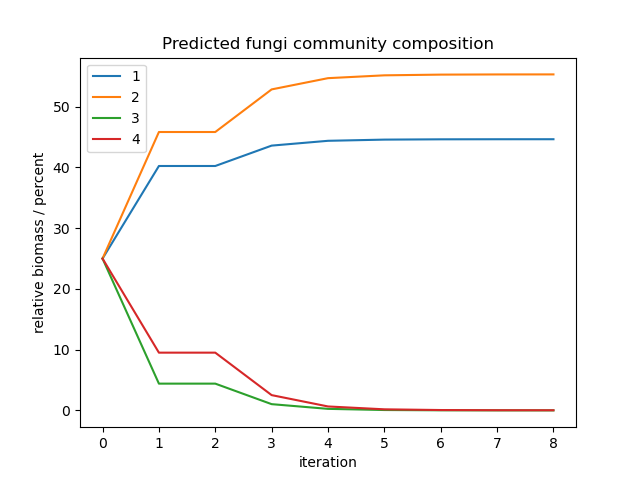
\includegraphics[width=\textwidth]{markov-4.png}
    \end{minipage}
    \begin{minipage}{0.4\textwidth}
        \caption{The community composition of a quad-species system, after several iteration, the relative biomass reaches homeostasis. 1 - Phlebia acerina, 2 - Phlebiopsis flavidoalba, 3 - Armillaria gallica, 4 - Armillaria tabescens}
    \end{minipage}
\end{figure}
